%%%%%%%% ICML 2025 EXAMPLE LATEX SUBMISSION FILE %%%%%%%%%%%%%%%%%

\documentclass{article}

% Recommended, but optional, packages for figures and better typesetting:
\usepackage{microtype}
\usepackage{graphicx}
\usepackage{subcaption}
\usepackage{booktabs} % for professional tables
% hyperref makes hyperlinks in the resulting PDF.
% If your build breaks (sometimes temporarily if a hyperlink spans a page)
% please comment out the following usepackage line and replace
% \usepackage{icml2025} with \usepackage[nohyperref]{icml2025} above.
\usepackage{hyperref}



% Attempt to make hyperref and algorithmic work together better:
\newcommand{\theHalgorithm}{\arabic{algorithm}}

% Use the following line for the initial blind version submitted for review:
\usepackage{icml2025}

% If accepted, instead use the following line for the camera-ready submission:
%\usepackage[accepted]{icml2025}

% For theorems and such
\usepackage{amsmath}
\usepackage{amssymb}
\usepackage{mathtools}
\usepackage{amsthm}

% if you use cleveref..
\usepackage[capitalize,noabbrev]{cleveref}

%%%%%%%%%%%%%%%%%%%%%%%%%%%%%%%%
% THEOREMS
%%%%%%%%%%%%%%%%%%%%%%%%%%%%%%%%
\theoremstyle{plain}
\newtheorem{theorem}{Theorem}[section]
\newtheorem{proposition}[theorem]{Proposition}
\newtheorem{lemma}[theorem]{Lemma}
\newtheorem{corollary}[theorem]{Corollary}
\theoremstyle{definition}
\newtheorem{definition}[theorem]{Definition}
\newtheorem{assumption}[theorem]{Assumption}
\theoremstyle{remark}
\newtheorem{remark}[theorem]{Remark}

% Todonotes is useful during development; simply uncomment the next line
%    and comment out the line below the next line to turn off comments
%\usepackage[disable,textsize=tiny]{todonotes}
\usepackage[textsize=tiny]{todonotes}


% The \icmltitle you define below is probably too long as a header.
% Therefore, a short form for the running title is supplied here:
\icmltitlerunning{Submission and Formatting Instructions for ICML 2025}

\begin{document}

\twocolumn[
\icmltitle{Dataset Distillation via Dynamic Difficulty Alignment}

% It is OKAY to include author information, even for blind
% submissions: the style file will automatically remove it for you
% unless you've provided the [accepted] option to the icml2025
% package.

% List of affiliations: The first argument should be a (short)
% identifier you will use later to specify author affiliations
% Academic affiliations should list Department, University, City, Region, Country
% Industry affiliations should list Company, City, Region, Country

% You can specify symbols, otherwise they are numbered in order.
% Ideally, you should not use this facility. Affiliations will be numbered
% in order of appearance and this is the preferred way.
\icmlsetsymbol{equal}{*}

\begin{icmlauthorlist}
\icmlauthor{Firstname1 Lastname1}{equal,yyy}
\icmlauthor{Firstname2 Lastname2}{equal,yyy,comp}
\icmlauthor{Firstname3 Lastname3}{comp}
\icmlauthor{Firstname4 Lastname4}{sch}
\icmlauthor{Firstname5 Lastname5}{yyy}
\icmlauthor{Firstname6 Lastname6}{sch,yyy,comp}
\icmlauthor{Firstname7 Lastname7}{comp}
%\icmlauthor{}{sch}
\icmlauthor{Firstname8 Lastname8}{sch}
\icmlauthor{Firstname8 Lastname8}{yyy,comp}
%\icmlauthor{}{sch}
%\icmlauthor{}{sch}
\end{icmlauthorlist}

\icmlaffiliation{yyy}{Department of XXX, University of YYY, Location, Country}
\icmlaffiliation{comp}{Company Name, Location, Country}
\icmlaffiliation{sch}{School of ZZZ, Institute of WWW, Location, Country}

\icmlcorrespondingauthor{Firstname1 Lastname1}{first1.last1@xxx.edu}
\icmlcorrespondingauthor{Firstname2 Lastname2}{first2.last2@www.uk}

% You may provide any keywords that you
% find helpful for describing your paper; these are used to populate
% the "keywords" metadata in the PDF but will not be shown in the document
\icmlkeywords{Machine Learning, ICML}

\vskip 0.3in
]

% this must go after the closing bracket ] following \twocolumn[ ...

% This command actually creates the footnote in the first column
% listing the affiliations and the copyright notice.
% The command takes one argument, which is text to display at the start of the footnote.
% The \icmlEqualContribution command is standard text for equal contribution.
% Remove it (just {}) if you do not need this facility.

%\printAffiliationsAndNotice{}  % leave blank if no need to mention equal contribution
\printAffiliationsAndNotice{\icmlEqualContribution} % otherwise use the standard text.

\begin{abstract}
Dataset distillation has emerged as a prominent area of research, aiming to compress large, original datasets into compact, lightweight synthetic datasets. Although existing works have shown their effectiveness on small scale datasets, they struggle to maintain performance on large scale datasets. Our analysis reveals that conventional dataset distillation methods have a bias towards generating synthetic images that mainly capture the easy samples of the real dataset. Although this bias is actually beneficial for small scale datasets, larger datasets require synthetic images to be diverse, capturing not only the easy samples, but also the hard samples of the real dataset. To this end, we propose a novel dataset distillation framework that generates synthetic images in multiple small segments, where each segment is distilled by matching a small portion of the whole dataset. Each portion is obtained by filtering out images prior to distillation, and each synthetic segment is distilled using a different set of images . This method facilitates the generation of diverse synthetic datasets that captures both easy and hard samples of the real dataset. Our experiments show that our method incorporated into existing frameworks show SOTA performance across a variety of large scale datasets, paving the way to make dataset distillation more scalable to larger datasets.
\end{abstract}

\section{Introduction}
\label{submission}

The increasing scale of datasets poses significant challenges for training machine
learning models, including high storage requirements, computational demands, and extensive
training times. Dataset distillation addresses these challenges by synthesizing a smaller
dataset from the original dataset, such that models trained on the synthetic dataset achieves
performance comparable to those trained on the original dataset. This technique has practical
applications in various domains. For example, in edge computing, where devices such as
smartphones and IoT sensors have limited storage and computational power, dataset distillation
enables efficient on-device training. Similarly, in federated learning, it reduces the amount of
data transmitted between devices and servers, thereby improving communication efficiency.

\begin{figure}[t]
    \centering
    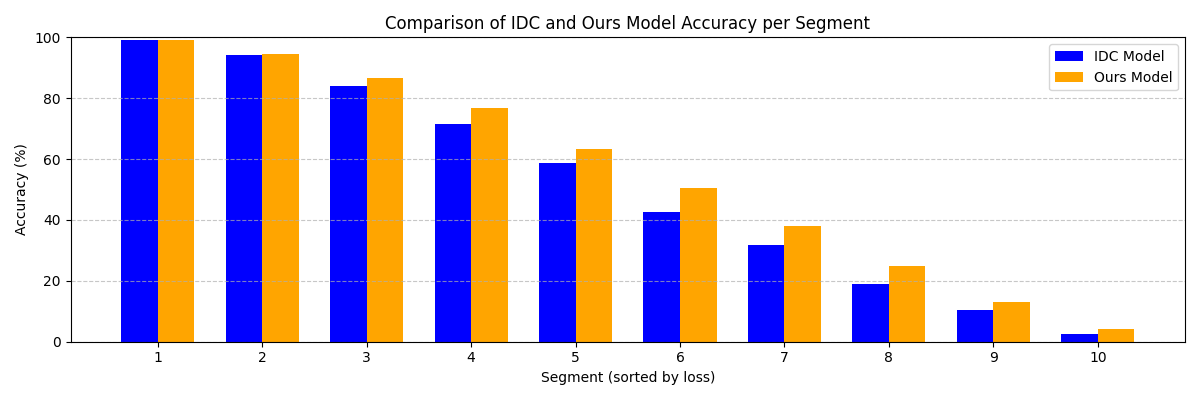
\includegraphics[width=0.5\textwidth]{./images/loss.png}
    \caption{Classification accuracy of a model trained with synthetic datasets generated using IDC and our method.
    The dataset is divided into 10 segments, ordered by loss. Segments on the left represent easy samples,
    while segments on the right represent hard samples. Performance quickly saturates
    for hard samples with IDC, while our method maintains high accuracy even for hard samples.}
    \label{fig:loss}
\end{figure}

Two main approaches to dataset distillation are gradient matching and trajectory matching. Gradient
matching optimizes the synthetic dataset to produce gradients similar to those of the original dataset,
while trajectory matching extends this idea by aligning the full training trajectories of the original dataset.
These methods have shown effectiveness in generating synthetic datasets with a small images-per-class (IPC).
However, their performance degrades when generating synthetic datasets with high IPC.
The primary reason for this limitation is that conventional methods are biased toward
generating synthetic datasets that primarily capture easy samples of the original dataset.
As illustrated in Fig.~\ref{fig:loss}, both IDC and MTT, the standard gradient matching and
trajectory matching methods, achieve high classification accuracy for easy samples but
exhibit significant performance degradation for harder samples.
Recent methods, such as DATM and SelMatch, have attempted to address the easy-sample bias by
embedding hard features into synthetic datasets. DATM achieves this by matching specific parts
of training trajectories, whereas SelMatch relies on heuristic scores to select
samples of appropriate difficulty for distillation.
However, these methods rely heavily on heuristics, requiring manual inspection and extensive
trial-and-error processes. This reliance poses a challenge as datasets vary in their
characteristics, necessitating separate adjustments for each dataset. Moreover, even within
the same dataset, additional tuning is often required for different IPC settings.
To address these challenges, we propose D4A (Dataset Distillation via Dynamic Difficulty Alignment),
a novel framework that dynamically incorporates hard samples into synthetic datasets without
relying on heuristic intervention. Instead of manual inspection, D4A employs
a model-driven approach to identify parts of the original dataset that should be embedded
into the synthetic dataset.
The process begins by generating a small subset of synthetic images.
A model trained on these synthetic images is then used to classify the original dataset.
Images that are correctly classified are identified as easy samples and discarded,
while misclassified images are retained as hard samples for embedding into the synthetic dataset.
This iterative filtering process ensures that subsequent synthetic images emphasize harder samples.
However, naively filtering out easy samples can lead to performance degradation due
to the forgetting phenomenon~\cite{}, where adding new synthetic images to the existing synthetic
dataset causes the trained model to misclassify images it previously classified correctly.
To mitigate forgetting, we design a regularization loss derived from previously generated
synthetic images. This loss is applied during the training of subsequent synthetic images,
reducing forgetting and improving overall performance.
Our main contributions can be summarized as follows:
\begin{itemize}
    \item We propose D4A, a novel dataset distillation framework that dynamically incorporates hard samples into synthetic datasets without heuristic intervention.  
    \item We introduce a regularization loss to mitigate the forgetting phenomenon, reducing misclassifications caused by the addition of new synthetic segments.  
    \item Our method achieves state-of-the-art performance across diverse datasets. For example, in the Tiny-ImageNet 50 IPC setting, D4A achieves 44.3\% accuracy, outperforming the previous best method by a margin of 4.6\%.  
\end{itemize}


\section{Related Works}
Dataset distillation compresses real images into synthetic images by optimizing the distance between the features of real and synthetic images.
Current research primarily focuses on two strategies: gradient/trajectory matching and distribution matching.

\textbf{Gradient/Trajectory Matching}: The core principle of these methods is that synthetic images should produce back-propagation signals similar to those of real images when training models.
DC~\cite{} proposes to match one-step gradients, while MTT~\cite{} advances this concept by matching entire training trajectories.
Although trajectory matching methods are often regarded as the current SOTA framework for dataset distillation, our experiments reveal that gradient matching methods outperform them on large-scale datasets and high-IPC settings.
Furthermore, gradient matching methods demonstrate superior generalization across multiple architectures, which is why we mainly implement our method to gradient matching frameworks.

\textbf{Distribution Matching}: An alternative approach involves aligning the feature maps of real and synthetic data.
Early methods such as CAFE and DM employed this strategy but showed inferior performance compared to gradient or trajectory matching frameworks.
Recent advances in this domain propose aligning the batch normalization statistics of real and synthetic images to generate synthetic data.
However, these methods are highly memory-intensive, requiring roughly 40 times more memory to store soft labels than synthetic images themselves.
Additionally, the synthetic images generated using this approach often perform worse than randomly selected images.
Given these limitations, we conclude that distribution matching methods are not well-suited for dataset distillation. Therefore, our work focuses on enhancing traditional gradient/trajectory matching approaches.

\section{Preliminary}

Dataset distillation is a task of generating a batch of synthetic images $\mathcal{S}$ such that networks trained with $\mathcal{S}$ perform similar to networks that are trained with the original training set $\mathcal{R}$. However, directly optimizing with respect to the generalization performance is very expensive, so surrogate objectives are solved instead to minimize distance between the real and synthetic dataset.

\begin{equation}
R: \text{Real Dataset}
\end{equation}
\begin{equation}
S: \text{Synthetic Dataset}
\end{equation}
\begin{equation}
S^* = \arg \min_{S} \mathcal{D}(S,R)
\end{equation}

The distance between the datasets can be measured in term of feature maps, gradients, or training trajectories. 

The  DASM framework can be implemented into all three surrogate objective methods, but as stated earlier, we work on gradient matching methods due to its superior performance and cross architecture generalization. In particular, we build upon IDC, where gradient matching is performed with downsampled synthetic images.

\begin{equation}
S^* = \arg \min_{S} \mathcal{D} \left( \nabla_{\theta} \mathcal{L}(\theta(\mathcal{A}^*(S))), \nabla_{\theta} \mathcal{L}(\theta(\mathcal{A}(R))) \right)
\end{equation}

$\mathcal{A}$ represents differential siamese augmentation, and $\mathcal{A}^*$ is upsampling followed by $\mathcal{A}$.






% In the unusual situation where you want a paper to appear in the
% references without citing it in the main text, use \nocite
\nocite{langley00}

\bibliography{example_paper}
\bibliographystyle{icml2025}


%%%%%%%%%%%%%%%%%%%%%%%%%%%%%%%%%%%%%%%%%%%%%%%%%%%%%%%%%%%%%%%%%%%%%%%%%%%%%%%
%%%%%%%%%%%%%%%%%%%%%%%%%%%%%%%%%%%%%%%%%%%%%%%%%%%%%%%%%%%%%%%%%%%%%%%%%%%%%%%
% APPENDIX
%%%%%%%%%%%%%%%%%%%%%%%%%%%%%%%%%%%%%%%%%%%%%%%%%%%%%%%%%%%%%%%%%%%%%%%%%%%%%%%
%%%%%%%%%%%%%%%%%%%%%%%%%%%%%%%%%%%%%%%%%%%%%%%%%%%%%%%%%%%%%%%%%%%%%%%%%%%%%%%
\newpage
\appendix
\onecolumn
\section{You \emph{can} have an appendix here.}

You can have as much text here as you want. The main body must be at most $8$ pages long.
For the final version, one more page can be added.
If you want, you can use an appendix like this one.  

The $\mathtt{\backslash onecolumn}$ command above can be kept in place if you prefer a one-column appendix, or can be removed if you prefer a two-column appendix.  Apart from this possible change, the style (font size, spacing, margins, page numbering, etc.) should be kept the same as the main body.
%%%%%%%%%%%%%%%%%%%%%%%%%%%%%%%%%%%%%%%%%%%%%%%%%%%%%%%%%%%%%%%%%%%%%%%%%%%%%%%
%%%%%%%%%%%%%%%%%%%%%%%%%%%%%%%%%%%%%%%%%%%%%%%%%%%%%%%%%%%%%%%%%%%%%%%%%%%%%%%


\end{document}


% This document was modified from the file originally made available by
% Pat Langley and Andrea Danyluk for ICML-2K. This version was created
% by Iain Murray in 2018, and modified by Alexandre Bouchard in
% 2019 and 2021 and by Csaba Szepesvari, Gang Niu and Sivan Sabato in 2022.
% Modified again in 2023 and 2024 by Sivan Sabato and Jonathan Scarlett.
% Previous contributors include Dan Roy, Lise Getoor and Tobias
% Scheffer, which was slightly modified from the 2010 version by
% Thorsten Joachims & Johannes Fuernkranz, slightly modified from the
% 2009 version by Kiri Wagstaff and Sam Roweis's 2008 version, which is
% slightly modified from Prasad Tadepalli's 2007 version which is a
% lightly changed version of the previous year's version by Andrew
% Moore, which was in turn edited from those of Kristian Kersting and
% Codrina Lauth. Alex Smola contributed to the algorithmic style files.
